\documentclass[]{article}
\usepackage{lmodern}
\usepackage{amssymb,amsmath}
\usepackage{ifxetex,ifluatex}
\usepackage{fixltx2e} % provides \textsubscript
\ifnum 0\ifxetex 1\fi\ifluatex 1\fi=0 % if pdftex
  \usepackage[T1]{fontenc}
  \usepackage[utf8]{inputenc}
\else % if luatex or xelatex
  \ifxetex
    \usepackage{mathspec}
  \else
    \usepackage{fontspec}
  \fi
  \defaultfontfeatures{Ligatures=TeX,Scale=MatchLowercase}
\fi
% use upquote if available, for straight quotes in verbatim environments
\IfFileExists{upquote.sty}{\usepackage{upquote}}{}
% use microtype if available
\IfFileExists{microtype.sty}{%
\usepackage{microtype}
\UseMicrotypeSet[protrusion]{basicmath} % disable protrusion for tt fonts
}{}
\usepackage[unicode=true]{hyperref}
\hypersetup{
            pdfborder={0 0 0},
            breaklinks=true}
\urlstyle{same}  % don't use monospace font for urls
\usepackage{graphicx,grffile}
\makeatletter
\def\maxwidth{\ifdim\Gin@nat@width>\linewidth\linewidth\else\Gin@nat@width\fi}
\def\maxheight{\ifdim\Gin@nat@height>\textheight\textheight\else\Gin@nat@height\fi}
\makeatother
% Scale images if necessary, so that they will not overflow the page
% margins by default, and it is still possible to overwrite the defaults
% using explicit options in \includegraphics[width, height, ...]{}
\setkeys{Gin}{width=\maxwidth,height=\maxheight,keepaspectratio}
\IfFileExists{parskip.sty}{%
\usepackage{parskip}
}{% else
\setlength{\parindent}{0pt}
\setlength{\parskip}{6pt plus 2pt minus 1pt}
}
\setlength{\emergencystretch}{3em}  % prevent overfull lines
\providecommand{\tightlist}{%
  \setlength{\itemsep}{0pt}\setlength{\parskip}{0pt}}
\setcounter{secnumdepth}{0}
% Redefines (sub)paragraphs to behave more like sections
\ifx\paragraph\undefined\else
\let\oldparagraph\paragraph
\renewcommand{\paragraph}[1]{\oldparagraph{#1}\mbox{}}
\fi
\ifx\subparagraph\undefined\else
\let\oldsubparagraph\subparagraph
\renewcommand{\subparagraph}[1]{\oldsubparagraph{#1}\mbox{}}
\fi

% set default figure placement to htbp
\makeatletter
\def\fps@figure{htbp}
\makeatother


\date{}

\begin{document}

\emph{Le fratture}

\emph{Introduzione}

Le fratture sono definite come delle \emph{soluzioni di continuità di un
segmento osseo}.

Ogni segmento osseo ha una sua resistenza: per generare una frattura
quindi l'entità del trauma deve superare i limiti di elasticità e di
resistenza del segmento osseo colpito.

Di fronte ad una frattura (ad esempio di un osso lungo come il femore)
si possono riconoscere:

\begin{itemize}
\item
  \textbf{Focolaio di frattura:} corrisponde alla sede anatomica della
  frattura
\item
  \textbf{Rima della frattura:} rappresenta l'andamento della linea di
  demarcazione fra due o più segmenti di osso fratturato
\item
  \textbf{Monconi della frattura:} segmenti principali dell'osso
  fratturato
\end{itemize}

\begin{quote}
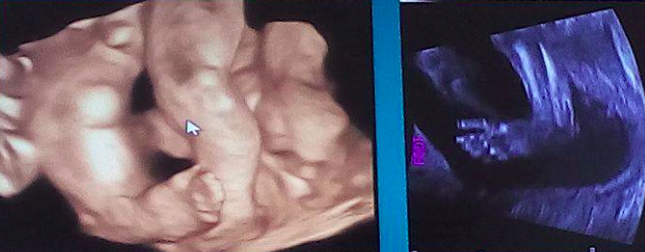
\includegraphics[width=6.64583in,height=4.19792in]{media/image1.png}

\emph{Classificazione}
\end{quote}

Le fratture possono essere classificate secondo diversi criteri.

\begin{quote}
\textbf{\emph{I.CLASSIFICAZIONE EZIOLOGIA}} (è la classificazione più
utilizzata) Dal punto di vista eziologico distinguiamo:

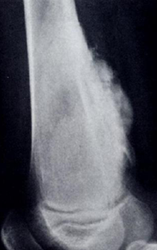
\includegraphics[width=2.67708in,height=1.95833in]{media/image2.png}
\end{quote}

\begin{itemize}
\item
  \textbf{Fratture traumatiche}: sono le fratture più frequenti e si
  verificano quando \emph{un \textbf{unico trauma efficiente} causa
  l'interruzione di un osso sano e strutturalmente normale.} Ad esempio
  se un motociclista urta contro un palo con conseguente frattura di
  tibia e perone allora definiremo quella come una frattura traumatica
  legata al trauma diretto della gamba contro il palo.
\item
  \textbf{Fratture da durata o da stress}: conseguenti \emph{a ripetuti
  \textbf{microtraumi non efficienti} che agiscono nel tempo su un osso
  sano}. Il cedimento strutturale è \emph{per sovraccarichi funzionali
  che superano i limiti di resistenza meccanica dell'osso stesso. Sono
  per definizione stessa delle fratture incomplete! Tuttavia se il
  meccanismo lesivo non viene interrotto, evolvono in vere e proprie
  fratture complete che coinvolgono principalmente gli arti inferiore
  dal momento che questi sono esposti a carichi di lavoro maggiori.}
  Possiamo prendere in considerazione diverse situazioni come ad esempio
  quella di un maratoneta che si allena costantemente e partecipa a 3/4
  maratone l'anno, può andare incontro ad una frattura da stress del
  metatarso. Altra frattura da stress comune è quella dei metacarpi nei
  pugili o del collo del femore o del piatto tibiale nei Marines (c'è
  molta letteratura al riguardo).
\item
  \textbf{Fratture patologiche}. Si tratta di una tipologia la cui
  incidenza è progressivamente aumentata negli ultimi anni. Si
  instaurano su un \emph{``osso patologico}'' cioè un osso che risulta
  essere più debole del normale e meccanicamente insufficiente. Molto
  spesso non è nemmeno presente l'evento traumatico o talvolta è un
  trauma inefficace. Le cause che portano ad un indebolimento dell'osso
  possono essere varie e ne vediamo alcune:
\end{itemize}

\begin{itemize}
\item
  \emph{Osteoporosi} ad esempio una persona anziana che si alza dalla
  sedia e accusa poi dolore alla schiena, può riportare una frattura dei
  corpi vertebrali su base osteoporotica. \emph{L'osteoporosi è definita
  come una riduzione della massa ossea con rarefazione delle trabecole
  nell'osso spongioso e assottigliamento della corticale che comporta un
  aumentato rischio di fratture. Va sottolineato che nell'osteoporosi la
  massa ossea è quantitativamente ridotta, ma qualitativamente normale
  perciò possono verificarsi fratture per traumi molto modesti come ad
  esempio al collo del femore o alle vertebre e nella maggior parte dei
  casi sono conseguenti a traumi multipli piuttosto che ad un unico
  trauma evidente.}
\end{itemize}

\begin{quote}
\textbf{N.B.:} Non abbiamo una definizione univoca per le fratture da
osteoporosi. Sul libro dice chiaramente che non sono classificabili come
fratture patologiche, ma nella lezione sulle fratture del collo del
femore (sulla vecchia dispensa Sigfied) il prof Ceccarelli le inserisce
tra le fratture patologiche ``border-line''. Durante questa lezione
(tenuta dal prof. Vaienti) sono riportate come esempio di fratture
patologiche e chiesti chiarimenti al prof., questi ribadisce che loro le
considerano come patologiche!
\end{quote}

\begin{itemize}
\item
  \emph{Malattie congenite} come ad esempio l'osteogenesi imperfetta
  (OI). \emph{Detta anche malattia delle ossa di vetro o malattie delle
  sclere blu, l'OI è una patologia che colpisce gli individui di sesso
  maschile principalmente ed è dovuta ad anomalie nella sintesi del
  collagene di tipo I con problemi a carico dello scheletro, delle
  articolazione, degli occhi (sclere blu), delle orecchie, della cute e
  dei denti. Può essere a penetranza più o meno completa e,
  conseguentemente, ad espressione clinica più o meno grave: oggi se ne
  conoscono sette tipologie a gravità diversa.}
\item
  \emph{Tumori:} sia tumori primitivi alle ossa come cisti ossee o
  tumori maligni primitivi sia metastasi di tumori in altre sedi tra cui
  più frequentemente tumore della mammella, del polmone, della prostata
  e dell'utero. \emph{Questi possono colpire tanto i bambini quanto gli
  adulti però nei bambini sono generalmente più benigni.}
\item
  \emph{Infezioni} come nel caso dell'osteomielite
\end{itemize}

N.B.Delle cause riportate ricordare che l'osteogenesi imperfetta è la
causa più ricorrente tra i bambini mentre l'osteoporosi tra gli anziani.
Le lesioni osteolitiche di natura neoplastica benigne o maligne,
primitive o secondarie riguardano principalmente gli adulti e anziano,
ma a volte anche i bambini

\begin{itemize}
\item
  \textbf{Fratture iatrogene} \textbf{o osteotomie chirurgiche}:
  interruzioni del tessuto osseo \emph{realizzate dal chirurgo a fini
  terapeutici quindi per correggere una deformità.} Possono essere
  realizzate manualmente o più frequentemente mediante l'utilizzo di
  strumenti chirurgici (seghe, fili, scalpelli, osteotomi). Ad esempio
  nel caso di ginocchio varo (è il cosiddetto ginocchio a parentesi:
  l'opposto del ginocchio a X o ginocchio valgo) viene trattato
  schematicamente così: con lo scalpello si effettua la frattura
  iatrogena quindi si corregge la deformità ed infine si blocca il tutto
  con una piastra e delle viti. Per l'osteotomia dell'anca finalizzata a
  correggere un'anca displasica (es. osteotomia di Salter, osteotomia di
  Chiari) si procede come di seguito: si frattura l'acetabolo, si
  riorienta nella posizione corretta e poi si blocca con delle viti.
  \emph{Infine l'osteotomia è eseguita anche per correggere eterometrie
  degli arti.} \emph{La calloclasia invece è l'interruzione chirurgica
  di un callo osseo che si effettua quando la frattura si sta riparando
  in modo inadeguato}
\end{itemize}

\begin{quote}
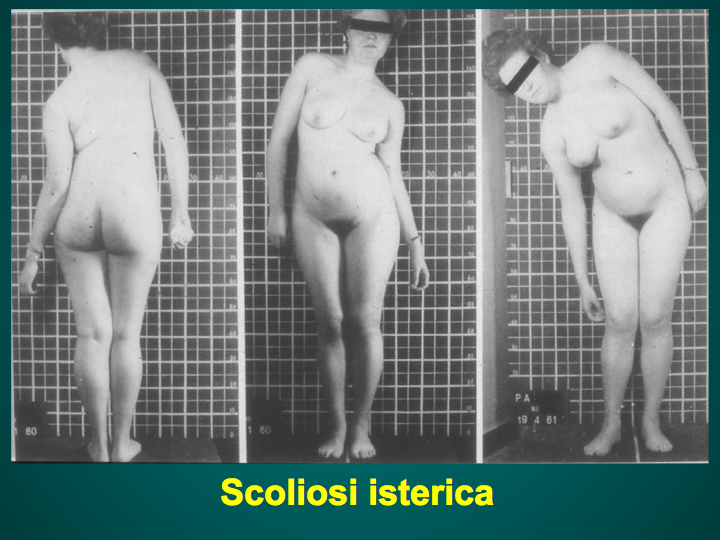
\includegraphics[width=3.88542in,height=2.81250in]{media/image3.png}
\end{quote}

\textbf{II. CLASSIFICAZIONE IN BASE AL TIPO DI TRAUMA}

\begin{itemize}
\item
  \textbf{Frattura per trauma diretto:} il trauma agisce nel punto
  stesso in cui si manista la frattura. Ad esempio un soggetto che
  riceva un calcio al terzo medio della tibia con conseguente frattura
  dell'osso in quel punto. \emph{Distingueremo in questo caso:}
\end{itemize}

\begin{itemize}
\item
  \emph{Fratture da urto}
\item
  \emph{Fratture da schiacciamento}
\item
  \emph{Fratture penetranti (o da arma da fuoco)}
\end{itemize}

\begin{itemize}
\item
  \textbf{Frattura per trauma indiretto:} in questo caso il trauma causa
  una frattura a distanza rispetto al punto di applicazione del trauma
  stesso. Ad esempio chi cade sulla mano, ma riporta una frattura del
  gomito. \emph{{[}La vecchia dispensa Sigfied suddivide ulteriormente
  la fratture indirette in fratture per torsione, per flessione, per
  compressione, per trazione e per azione combinata. Nella lezione il
  prof non riporta tale sub classificazione e procede con la
  classificazione in base al meccanismo lesivo che coincide con tale sub
  classificazione riportata nella vecchia dispensa{]}}
\end{itemize}

.

\textbf{III. CLASSIFICAZIONE IN BASE AL MECCANISMO LESIVO}

\begin{itemize}
\item
  \textbf{Fratture da flessione:} il trauma determina una modifica della
  normale curvatura dell'osso fino alla rottura. \emph{Ad esempio le
  ginnaste che flettono troppo l'ulna.}
\item
  \textbf{Fratture da torsione:} in questo caso il trauma è di tipo
  torcente rispetto all'asse osso. \emph{Ad esempio se metto il piede
  tra il marciapiede e un altro ostacolo, il piedi si incastrerà e cadrò
  in avanti: si produce una rima di frattura spiroide.}
\item
  \textbf{Fratture da compressione o da schiacciamento:} \emph{l'esempio
  tipico è a livello dell'osso spongioso vertebrale}
\item
  \textbf{Fratture da strappamento:} in questo caso la trazione di un
  legamento o di un tendine causa il distacco dell'osso che ivi si
  inserisce\emph{.} Ad esempio a volte il legamento rotuleo ``strappa
  l'osso a livello della sua inserzione sulla tuberosità tibiale
  anteriore
\item
  \emph{\textbf{Fratture per azione combinata}}
\end{itemize}

\textbf{IV. CLASSIFICAZIONE IN BASE AL DECORSO DELLA RIMA}

\begin{itemize}
\item
  \textbf{Fratture trasversali:} la rima è ad \emph{angolo retto}
  rispetto all'asse longitudinale dell'osso
\item
  \textbf{Fratture oblique:} la rima forma un \emph{angolo minore di
  90°} rispetto all'asse longitudinale
\item
  \textbf{Fratture spiroidi:} la rima compie un \emph{decorso a spirale}
  rispetto al segmento osseo
\item
  \textbf{Fratture longitudinali:} la rima è \emph{parallela} all'asse
  longitudinale dell'osso
\end{itemize}

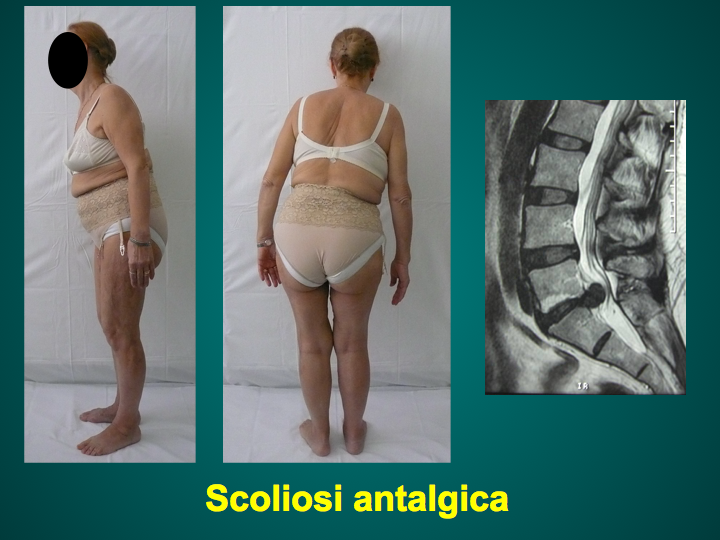
\includegraphics[width=3.34375in,height=2.00000in]{media/image4.png}
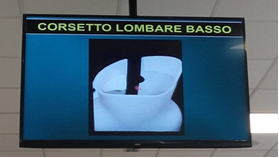
\includegraphics[width=3.65625in,height=2.78125in]{media/image5.png}

\begin{quote}
\textbf{V. CLASSIFICAZIONE PER SPOSTAMENTO DEI MONCONI}
\end{quote}

\begin{itemize}
\item
  \textbf{Fratture composte:} i frammenti \emph{conservano} la loro
  posizione e rapporti anatomici \emph{così da non modificare la normale
  configurazione dell'osso.}
\item
  \textbf{Fratture scomposte:} i frammenti \emph{non conservano} la loro
  posizione anatomica \emph{e la forma del segmento scheletrico appare
  alterata dallo spostamento dei frammenti stessi. Per la diafisi delle
  ossa lunghe si descrivono 4 tipi di scomposizione}
\end{itemize}

\begin{itemize}
\item
  \emph{Longitudinale:} i monconi si sovrappongono in lunghezza l'uno
  sull'altro
\item
  \emph{Angolare:} i monconi si angolano l'uno rispetto all'altro
\item
  \emph{Laterale:} i monconi non si sovrappongono, ma sono spostati
  lateralmente l'uno rispetto all'altro
\item
  \emph{Rotatorio:} i monconi ruotano l'uno sull'altro
\end{itemize}

\begin{itemize}
\item
  \textbf{Fratture scomposte e ingranate:} i monconi si ingranano l'uno
  sull'altro. Generalmente sono dovute a traumi da compressione. Una
  frattura scomposta ed ingranata dei corpi vertebrali, si riconosce
  all'RX perché normalmente il corpo vertebrale appare di forma
  rettangolare mentre in caso di frattura ingranata il rettangolo
  scompare e si vede una cuneizzazione perché la parte anteriore si
  schiaccia rispetto a quella posteriore
\end{itemize}

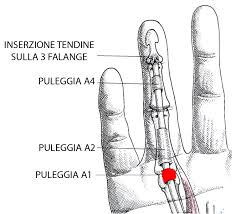
\includegraphics[width=6.03125in,height=3.62500in]{media/image6.png}

\textbf{VI. CLASSIFICAZIONE PER NUMERO DI FRAMMENTI}

\begin{itemize}
\item
  \textbf{Fratture unifocali:} una rima di frattura e due monconi
\item
  \textbf{Fratture bifocali:} due focolai di frattura posti a livelli
  diversi e tre monconi
\item
  \textbf{Fratture plurifocali o pluriframmentarie:} tanti focolai di
  frattura e tanti monconi.
\end{itemize}

\textbf{VII. CLASSIFICAZIONE PER SEDE SCHELETRICE (per ossa lunghe)}

\begin{itemize}
\item
  \textbf{Fratture diafisarie} (la diafisi è la parte centrale di un
  osso lungo)
\item
  \textbf{Fratture epifisarie} (l'epifisi è la parte articolare distale
  di un osso lungo)
\item
  \textbf{Fratture metafisarie} (la metafisi è a metà tra epifisi e
  diafisi)
\end{itemize}

\textbf{VIII. CLASSIFICAZIONE PER ALTRA SEDE (no sede scheletrica!) }

È la classificazione più comunemente riportata nei referti:

\begin{itemize}
\item
  \textbf{Frattura articolare:} \emph{la rima di frattura intacca la
  cartilagine articolare}. Caratterizzata da una prognosi peggiore
  legata alla maggiore frequenza di insorgenza di artrosi post-
  traumatica; per scongiurare tale evoluzione si cerca di ripristinare
  un piano cartilagineo il più normale possibile tuttavia molto spesso
  la cartilagine è troppo rovinata oppure risulta impossibile rimetterla
  a posto quindi si lasciano degli scalini di incongruenza.
\item
  \textbf{Frattura extra-articolare:} la rima di frattura non arriva a
  livello della cartilagine articolare e questo generalmente si associa
  ad una prognosi migliore perché non c'è rischio di artrosi
  post-traumatica. \emph{Queste sono ulteriormente suddivise in:}
\end{itemize}

\begin{itemize}
\item
  \emph{Intra-capsulari: sono generalmente piuttosto gravi perché spesso
  vanno incontro a devascolarizzazione e il danno vascolare limita la
  capacità di creare un callo osseo}
\item
  \emph{Extra- capsulari}
\end{itemize}

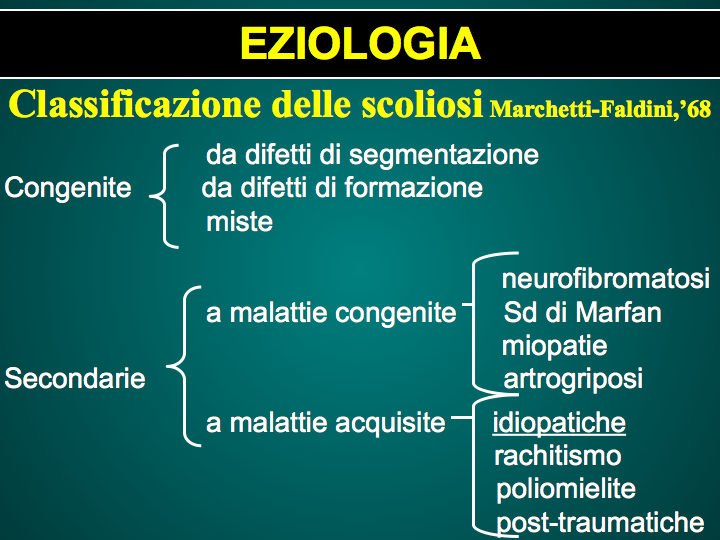
\includegraphics[width=5.58333in,height=4.07292in]{media/image7.png}

\textbf{IX. CLASSIFICAZIONE PER ENTITA' DEL DANNO}

\begin{itemize}
\item
  \textbf{Fratture complete:} interessano \emph{tutta la circonferenza}
  dell'osso
\item
  \textbf{Fratture incomplete:} \emph{non} interessano tutta la
  circonferenza. Possono essere a loro volta ulteriormente suddivise in:
\end{itemize}

\begin{itemize}
\item
  Fratture per infrazione
\item
  Fratture ``a legno verde'': questa espressione viene generalmente
  utilizzata quando si è di fronte ad una frattura in un bambino poiché
  in questo caso le loro ossa lunghe sono più plastiche rispetto a
  quelle di un adulto e quindi sono esposte ad un minor rischio di
  frattura. In questo caso avremo uno sfibramento o una piegatura, ma
  non una rottura dell'osso da cui il paragone con il legno verde che ha
  bisogno di una stimolazione più forte per spezzarsi rispetto ad un
  legno secco.
\end{itemize}

\begin{quote}
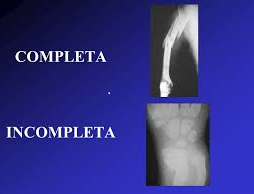
\includegraphics[width=2.64583in,height=2.02083in]{media/image8.png}
\end{quote}

\textbf{X. CLASSIFICAZIONE IN BASE ALL'INTEGRITA' DEL MANTELLO CUTANEO}

Si tratta di una classificazione molto importante per gli ortopedici

\begin{quote}
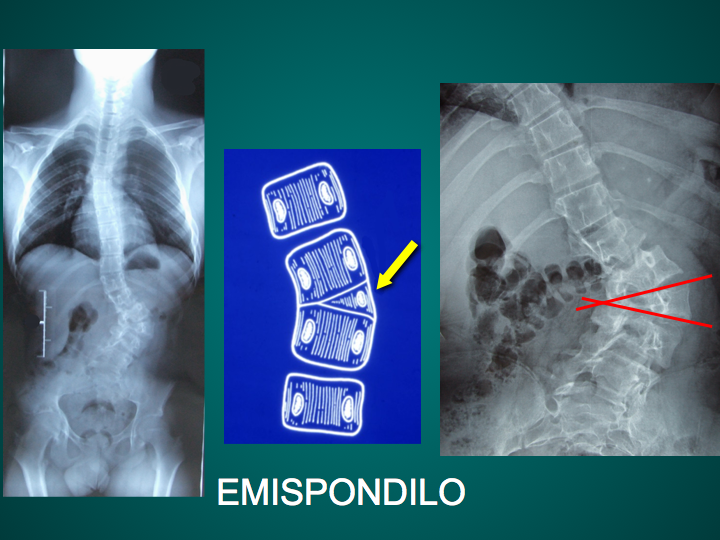
\includegraphics[width=2.39583in,height=2.28125in]{media/image9.png}
\end{quote}

\begin{itemize}
\item
  \textbf{CHIUSE}: attorno alla rima di frattura e ai monconi \emph{la
  cute è integra}
\item
  \textbf{ESPOSTE (O APERTE)} = \emph{l'integrità cutanea è interrotta}
  e il focolaio di frattura comunica con l'ambiente esterno tramite una
  ferita più o meno ampia. \emph{In questo caso il focolaio della
  frattura è esposto a contaminazione microbica che può evolvere verso
  una vera e propria osteomielite.} Sono molto importanti perché
  rappresentano delle urgenze chirurgiche.
\end{itemize}

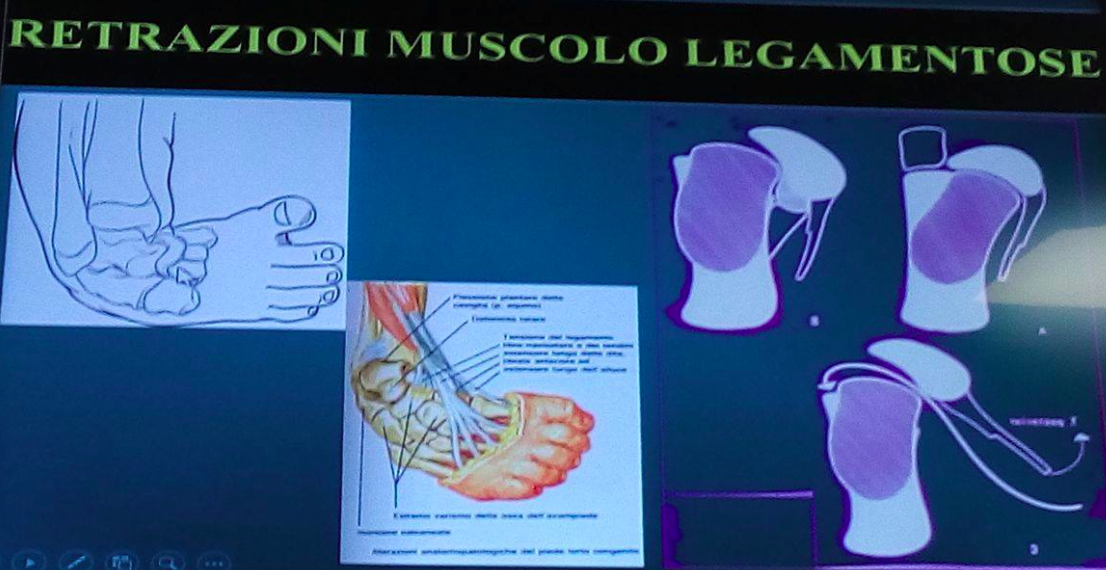
\includegraphics[width=5.41667in,height=3.25000in]{media/image10.png}

\emph{Urgenze}

\begin{itemize}
\item
  \textbf{Fratture esposte}: devono essere portate in sala operatoria
  massimo entro 6/8 ore (tempo minimo oltre il quale può insorgere
  infezione. L'infezione all'osso è difficilissima da trattare perché
  l'osso è già di per sé un tessuto a cui arriva poco sangue e in uno
  danneggiato ne arriva ancora meno). Nel minor tempo possibile
  l'ortopedico deve pulire il focolaio, rimuovere i tessuti necrotici,
  stabilizzare con un fissatore a ponte e coprire il più possibile con
  muscoli, sottocute e cute la ferita.
\item
  \textbf{Distacchi epifisari}: parliamo di distacco epifisario quando,
  nei bambini e nei giovani adulti, si osserva la separazione traumatica
  dell'epifisi dalla metafasi alla quale aderisce per interposizione
  della cartilagine di accrescimento (la rima di frattura passa
  attraverso la cartilagine di accrescimento). Ricordate che il tessuto
  cartilagineo fertile guida l'accrescimento delle ossa lunghe. Possono
  essere distinti in:
\end{itemize}

\begin{itemize}
\item
  \textbf{Puri}: è interessata \emph{solo} la cartilagine di
  accrescimento.
\item
  \textbf{Misti:} la rima di frattura di estende al tessuto contiguo
  perciò sono interessate la cartilagine di accrescimento e la
  cartilagine sopra e/o sottostante.
\end{itemize}

\begin{quote}
Anche queste devono essere stabilizzate entro 6/8 ore,
l\textbf{'}obiettivo è quello di agire il prima possibile per evitare la
morte delle cellule della zona di accrescimento. Non è prevedibile se
l'accrescimento avverrà poi in maniera normale oppure no, con i genitori
bisogna essere sempre molto schietti e diretti: si vedrà nel tempo cosa
accadrà.

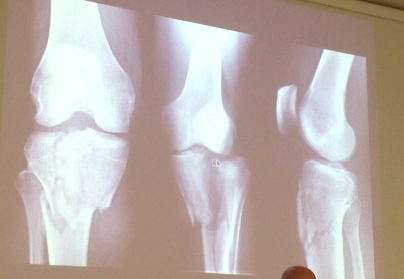
\includegraphics[width=3.73958in,height=2.86458in]{media/image11.png}
\end{quote}

\emph{La classificazione di Salter- Harris prevede la distinzione dei
distacchi epifisari in 5 tipi, in rapporto al decorso della rima di
frattura}

\begin{quote}
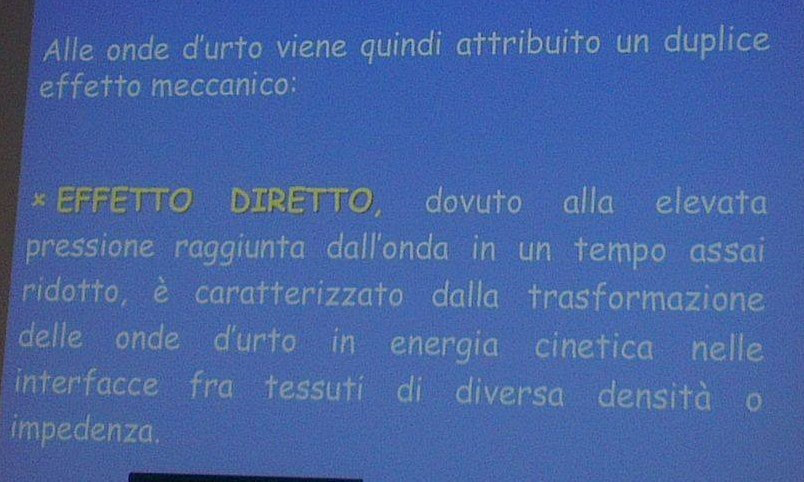
\includegraphics[width=4.06458in,height=3.46875in]{media/image12.jpeg}

Possibili inconvenienze in caso di distacchi epifisari possono essere:
\end{quote}

\begin{itemize}
\item
  Ipometria (un arto cresce meno dell'altro)
\item
  Distorcimento (un arto cresce storto)
\end{itemize}

\begin{itemize}
\item
  \textbf{FRATTURA-LUSSAZIONE}: Definiamo la lussazione come una perdita
  \emph{permanente} dei rapporti tra due capi articolari (il classico
  esempio è quando un soggetto cade e si ha lussazione della spalla: si
  dice che la spalla ``esce'' e non si riesce a ``rimetterla dentro'').
  La lussazione è da differenziare invece dalla distorsione definita
  come una perdita \emph{temporanea} dei rapporti tra due capi
  articolari.
\end{itemize}

Le lussazioni sono delle emergenze e devono essere trattate applicando
una trazione per rimettere a posto i capi articolari. Quando siamo di
fronte ad una lussazione prima di fare qualsiasi manovra dobbiamo sempre
eseguire un RX per valutare la possibilità che ci sia anche una
frattura. L'RX va sempre eseguita anche dopo la manovra di trazione.

\emph{Diagnosi}

Di fronte ad un sospetto clinico di frattura bisogna fare una diagnosi:
in prima battuta una diagnosi clinica che dovrà poi essere confermata
con delle indagini strumentali.

\textbf{Diagnosi clinica}:

Di fronte ad un sospetto di frattura avremo:

\begin{itemize}
\item
  \textbf{Segni di probabilità}
\end{itemize}

\begin{itemize}
\item
  \emph{Atteggiamento} ad esempio l'extra-rotazione e accorciamento
  della gamba indicano una possibile frattura del femore
\item
  \emph{Deformità} ad esempio il dorso a forchetta nella frattura di
  polso
\end{itemize}

\begin{quote}
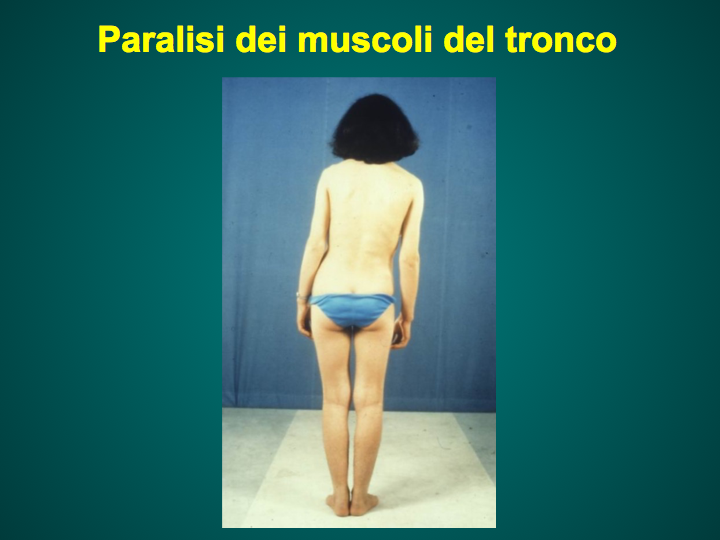
\includegraphics[width=4.77083in,height=2.91667in]{media/image13.png}
\end{quote}

\begin{itemize}
\item
  \emph{Ferite/ ecchimosi}
\item
  \emph{Tumefazioni e lesioni cutanee}
\item
  \emph{Dolore importante}
\item
  \emph{Impotenza funzionale} ad esempio il paziente non riesce a
  muovere l'arto interessato o a camminare
\end{itemize}

\begin{itemize}
\item
  \textbf{Segni di certezza }
\end{itemize}

\begin{itemize}
\item
  \emph{Crepitio}: dovuto ai due monconi di frattura che stridono l'uno
  sull'altro.
\item
  \emph{Motilità preternaturale} ad esempio prendo in mano un arto e
  vedo che si piega in maniera innaturale).
\end{itemize}

\begin{quote}
La diagnosi clinica deve poi essere sempre confermata dalle indagini
strumentali che permettono di poter pianificare un corretto trattamento
e che sono molto importanti dal punto di vista medico-legale. Le
principali sono:
\end{quote}

\begin{itemize}
\item
  \emph{RX STANDARD}: da eseguire in tutte le posizioni
  (antero-laterale, latero-laterale e obliqua) per avere una visione
  completa della frattura. È un esame che si deve eseguire SEMPRE nel
  sospetto di una frattura e molto spesso è dirimente.
\item
  \emph{TAC}: si esegue quando l'RX è negativa, ma il sospetto clinico
  di frattura è ancora fortemente presente (ad esempio quando c'è un
  dolore importante). A volte può far vedere delle fratture che con una
  normale RX non si vedono.
\end{itemize}

\begin{quote}
Viene anche richiesta per uno studio morfologico della frattura e per un
pianificazione pre-operatoria.

Non si esegue nei bambini perché utilizza radiazioni ionizzanti.
\end{quote}

\begin{itemize}
\item
  \emph{RMN}: utilizzata nei bambini al posto della TAC anche se risulta
  essere meno sensibile e meno specifica di quest'ultima. Rappresenta un
  ottimo mezzo per scoprire le fratture da stress.
\item
  \emph{SCINTIGRAFIA:} caduta completamente in disuso con l'introduzione
  della RMN.
\end{itemize}

\end{document}
